\documentclass[12pt,tikz,border=8pt]{standalone}
\usepackage{libertine}
\usepackage{amsmath,amssymb}
\usepackage{tikz}
\usetikzlibrary{arrows.meta}

\begin{document}
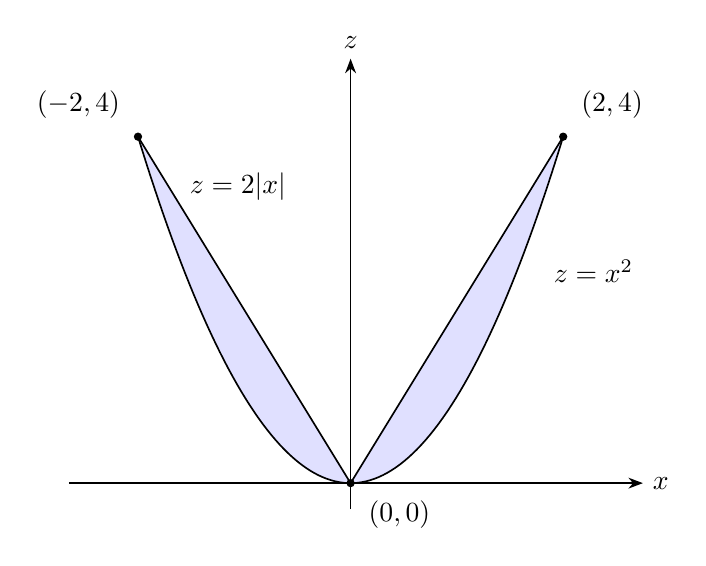
\begin{tikzpicture}[x=1.35cm,y=1.1cm,>=Stealth,
  boundary/.style={black,line width=0.6pt},
  every node/.style={font=\normalsize}]
  % The full xz-section has two lobes: x^2 <= z <= 2|x|.
  \fill[blue!12]
    (0,0) -- (2,4)
    plot[domain=2:0,samples=70] (\x,{\x*\x}) -- cycle;
  \fill[blue!12]
    (0,0) -- (-2,4)
    plot[domain=-2:0,samples=70] (\x,{\x*\x}) -- cycle;

  \draw[->,line width=0.5pt] (-2.65,0) -- (2.75,0)
    node[right] {$x$};
  \draw[->,line width=0.5pt] (0,-0.3) -- (0,4.9)
    node[above] {$z$};

  \draw[boundary] (-2,4) -- (0,0) -- (2,4);
  \draw[boundary,domain=-2:2,samples=100]
    plot (\x,{\x*\x});

  \fill (-2,4) circle[radius=1.5pt]
    node[above left=3pt] {$(-2,4)$};
  \fill (2,4) circle[radius=1.5pt]
    node[above right=3pt] {$(2,4)$};
  \fill (0,0) circle[radius=1.5pt]
    node[below right=3pt] {$(0,0)$};

  \node[above] at (-1.06,3.15) {$z=2|x|$};
  \node[right] at (1.82,2.45) {$z=x^2$};
\end{tikzpicture}
\end{document}
